% Options for packages loaded elsewhere
\PassOptionsToPackage{unicode}{hyperref}
\PassOptionsToPackage{hyphens}{url}
\PassOptionsToPackage{dvipsnames,svgnames,x11names}{xcolor}
%
\documentclass[
  letterpaper,
  DIV=11,
  numbers=noendperiod]{scrartcl}

\usepackage{amsmath,amssymb}
\usepackage{iftex}
\ifPDFTeX
  \usepackage[T1]{fontenc}
  \usepackage[utf8]{inputenc}
  \usepackage{textcomp} % provide euro and other symbols
\else % if luatex or xetex
  \usepackage{unicode-math}
  \defaultfontfeatures{Scale=MatchLowercase}
  \defaultfontfeatures[\rmfamily]{Ligatures=TeX,Scale=1}
\fi
\usepackage{lmodern}
\ifPDFTeX\else  
    % xetex/luatex font selection
\fi
% Use upquote if available, for straight quotes in verbatim environments
\IfFileExists{upquote.sty}{\usepackage{upquote}}{}
\IfFileExists{microtype.sty}{% use microtype if available
  \usepackage[]{microtype}
  \UseMicrotypeSet[protrusion]{basicmath} % disable protrusion for tt fonts
}{}
\makeatletter
\@ifundefined{KOMAClassName}{% if non-KOMA class
  \IfFileExists{parskip.sty}{%
    \usepackage{parskip}
  }{% else
    \setlength{\parindent}{0pt}
    \setlength{\parskip}{6pt plus 2pt minus 1pt}}
}{% if KOMA class
  \KOMAoptions{parskip=half}}
\makeatother
\usepackage{xcolor}
\setlength{\emergencystretch}{3em} % prevent overfull lines
\setcounter{secnumdepth}{-\maxdimen} % remove section numbering
% Make \paragraph and \subparagraph free-standing
\ifx\paragraph\undefined\else
  \let\oldparagraph\paragraph
  \renewcommand{\paragraph}[1]{\oldparagraph{#1}\mbox{}}
\fi
\ifx\subparagraph\undefined\else
  \let\oldsubparagraph\subparagraph
  \renewcommand{\subparagraph}[1]{\oldsubparagraph{#1}\mbox{}}
\fi


\providecommand{\tightlist}{%
  \setlength{\itemsep}{0pt}\setlength{\parskip}{0pt}}\usepackage{longtable,booktabs,array}
\usepackage{calc} % for calculating minipage widths
% Correct order of tables after \paragraph or \subparagraph
\usepackage{etoolbox}
\makeatletter
\patchcmd\longtable{\par}{\if@noskipsec\mbox{}\fi\par}{}{}
\makeatother
% Allow footnotes in longtable head/foot
\IfFileExists{footnotehyper.sty}{\usepackage{footnotehyper}}{\usepackage{footnote}}
\makesavenoteenv{longtable}
\usepackage{graphicx}
\makeatletter
\def\maxwidth{\ifdim\Gin@nat@width>\linewidth\linewidth\else\Gin@nat@width\fi}
\def\maxheight{\ifdim\Gin@nat@height>\textheight\textheight\else\Gin@nat@height\fi}
\makeatother
% Scale images if necessary, so that they will not overflow the page
% margins by default, and it is still possible to overwrite the defaults
% using explicit options in \includegraphics[width, height, ...]{}
\setkeys{Gin}{width=\maxwidth,height=\maxheight,keepaspectratio}
% Set default figure placement to htbp
\makeatletter
\def\fps@figure{htbp}
\makeatother

% TODO: Add custom LaTeX header directives here
\KOMAoption{captions}{tableheading}
\makeatletter
\makeatother
\makeatletter
\makeatother
\makeatletter
\@ifpackageloaded{caption}{}{\usepackage{caption}}
\AtBeginDocument{%
\ifdefined\contentsname
  \renewcommand*\contentsname{Table of contents}
\else
  \newcommand\contentsname{Table of contents}
\fi
\ifdefined\listfigurename
  \renewcommand*\listfigurename{List of Figures}
\else
  \newcommand\listfigurename{List of Figures}
\fi
\ifdefined\listtablename
  \renewcommand*\listtablename{List of Tables}
\else
  \newcommand\listtablename{List of Tables}
\fi
\ifdefined\figurename
  \renewcommand*\figurename{Figure}
\else
  \newcommand\figurename{Figure}
\fi
\ifdefined\tablename
  \renewcommand*\tablename{Table}
\else
  \newcommand\tablename{Table}
\fi
}
\@ifpackageloaded{float}{}{\usepackage{float}}
\floatstyle{ruled}
\@ifundefined{c@chapter}{\newfloat{codelisting}{h}{lop}}{\newfloat{codelisting}{h}{lop}[chapter]}
\floatname{codelisting}{Listing}
\newcommand*\listoflistings{\listof{codelisting}{List of Listings}}
\makeatother
\makeatletter
\@ifpackageloaded{caption}{}{\usepackage{caption}}
\@ifpackageloaded{subcaption}{}{\usepackage{subcaption}}
\makeatother
\makeatletter
\@ifpackageloaded{tcolorbox}{}{\usepackage[skins,breakable]{tcolorbox}}
\makeatother
\makeatletter
\@ifundefined{shadecolor}{\definecolor{shadecolor}{rgb}{.97, .97, .97}}
\makeatother
\makeatletter
\makeatother
\makeatletter
\makeatother
\ifLuaTeX
  \usepackage{selnolig}  % disable illegal ligatures
\fi
\IfFileExists{bookmark.sty}{\usepackage{bookmark}}{\usepackage{hyperref}}
\IfFileExists{xurl.sty}{\usepackage{xurl}}{} % add URL line breaks if available
\urlstyle{same} % disable monospaced font for URLs
\hypersetup{
  pdftitle={Tikken, scrollen, blowen.},
  pdfauthor={F.R. Bouwman; H.Jonkman},
  pdfkeywords={cannabis use, social media, online exposure, young
adults, DNERM, moderation analysis},
  colorlinks=true,
  linkcolor={blue},
  filecolor={Maroon},
  citecolor={Blue},
  urlcolor={Blue},
  pdfcreator={LaTeX via pandoc}}

\title{Tikken, scrollen, blowen.}
\usepackage{etoolbox}
\makeatletter
\providecommand{\subtitle}[1]{% add subtitle to \maketitle
  \apptocmd{\@title}{\par {\large #1 \par}}{}{}
}
\makeatother
\subtitle{De rol van online blootstelling op cannabisgebruik bij
jongeren en de mogelijke invloed van twee moderatoren}
\author{F.R. Bouwman \and H.Jonkman}
\date{}

\begin{document}
\maketitle
\begin{abstract}
Recently, cannabis use among young adults has increased dramatically.
This particular age group (16 -- 24 years) is vulnerable as cannabis use
during this period can have injurious consequences for mental health
(such as depression and suicidality), work and education. Based on the
Developmental Neuro-Ecological Risk-Taking Model (DNERM), it is assumed
that young individuals who are digitally exposed to risk behavior are
more likely to actually engage in such behavior themselves. Therefore,
this study investigated, through cross-sectional research, whether
online exposure to cannabis influences actual use. In addition, the
moderating role of social media frequency and parental cannabis use on
this potential relationship were analyzed. Participants (\(N\) = 153;
\(M_age\) = 21.8 years; 75.2\% girls) completed a questionnaire about
cannabis use, social media and choice behavior related to eating habits,
risk-taking and alcohol use. The results of the regression analyses
showed a small positive significant effect, which means the more
frequently someone is exposed to cannabis online, the more likely they
are to actually use cannabis. The results of the moderator analysis
showed that a moderate to high level of parental cannabis use
strengthened the examined relationship, while social media frequency did
not emerge as a significant predictor at all. The findings highlight the
influence of social media on cannabis use of young adults. It is
imperative to focus on raising awareness among parents and implementing
preventive measures to address the potential harmful consequences of
cannabis use.
\end{abstract}
\ifdefined\Shaded\renewenvironment{Shaded}{\begin{tcolorbox}[boxrule=0pt, borderline west={3pt}{0pt}{shadecolor}, interior hidden, enhanced, breakable, sharp corners, frame hidden]}{\end{tcolorbox}}\fi

\renewcommand*\contentsname{Table of contents}
{
\hypersetup{linkcolor=}
\setcounter{tocdepth}{3}
\tableofcontents
}
\hypertarget{introductie}{%
\section{Introductie}\label{introductie}}

Cannabis, ook wel bekend als marihuana, is wereldwijd de meest
geconsumeerde (illegale) drug (Amiet et al., 2020). Daarnaast neemt dit
cannabisgebruik de laatste jaren enorm toe, vooral onder jongvolwassenen
(Hall \& Degenhardt, 2009; Hall \& Degenhardt, 2013; Europees
Waarnemingscentrum voor drugs en drugsverslaving, 2019). In Nederland
heeft 26.1\% van de jongvolwassenen van 20 tot 24 jaar cannabis gebruikt
in het afgelopen jaar en 23,5\% van de jongeren van 18 en 19 jaar
(Nationale Drug Monitor, 2023). Deze cijfers zijn zorgelijk, aangezien
deze leeftijdscategorie een bijzonder kwetsbare groep vormt, waarbij
belangrijke biologische, sociale en persoonlijke overgangen en
veranderingen plaatsvinden die hun ontwikkeling beïnvloeden (Hall et
al., 2020). Blootstelling aan cannabis kan in deze adolescentieperiode
schadelijke gevolgen hebben voor de geestelijke gezondheid (o.a.
depressie en suïcidaliteit), werk en opleiding (Fergusson \& Boden,
2008; Lee et al., 2015). Naast het toenemende cannabisgebruik onder
jongvolwassenen groeit ook het gebruik van sociale media. Wereldwijd
zijn er momenteel 4.57 miljard internetgebruikers, waarvan er 3.81
miljard actief sociale media gebruiken (Starri, 2020). Sociale media
zijn een groot en betekenisvol deel geworden van het huidige dagelijks
leven, waarbij Facebook, YouTube, WhatsApp en Instagram momenteel het
meest gebruikt worden (Valkenburg, 2021; Starri, 2020). De platforms
worden onder andere gebruikt om op privégebied te interacteren met
familieleden en vrienden, maar ook publiekelijk met grotere groepen
vrienden, kennissen en collega's (Bayer et al., 2020). Echter, er is ook
steeds meer erkenning gekomen voor de veronderstelling dat sociale media
ook een negatieve impact kunnen hebben (Berryman et al., 2018). Het
biedt ruimte voor blootstelling aan riskant gedrag en de bijbehorende
reactie en houding van anderen ten opzichte van dat gedrag (Branley-Bell
\& Covey, 2017). Gesuggereerd wordt dat mensen die online blootgesteld
worden aan dat gedrag ook vaker betrokken zijn bij riskant gedrag in de
werkelijkheid, zoals drugsgebruik, overmatig alcoholgebruik, geweld en
ongeordend eten. Aangezien sociale media een steeds belangrijkere
opvoedingscontext blijken, wordt een eventuele relatie tussen digitale
blootstelling en risicogedrag gesuggereerd. Aansluitend op de
eerdergenoemde bevindingen van Branley-Bell \& Covey (2017) stelt het
Developmental Neuro-Ecological Risk-Taking Model (DNERM; Defoe, 2021)
ook dat jongeren die online blootgesteld worden aan risicogedrag eerder
en sneller daadwerkelijk risicogedrag vertonen. Op basis van deze recent
ontwikkelde theorie is de huidige studie opgezet omwille van de
zorgelijke cijfers van cannabisgebruik onder jongvolwassenen en de
kwetsbare groep die zij vormen. In dit onderzoek wordt de eventuele
relatie tussen digitale blootstelling aan cannabis en het daadwerkelijke
gebruik van cannabis of de intentie daartoe, onder jongeren van 16 tot
en met 24 jaar geanalyseerd. Tevens wordt onderzocht of de frequentie
van het sociale media gebruik van jongeren en/of het cannabisgebruik van
ouders invloed hebben op deze eventuele relatie.

\hypertarget{cannabisgebruik-onder-jongeren}{%
\subsection{Cannabisgebruik onder
jongeren}\label{cannabisgebruik-onder-jongeren}}

\hypertarget{cannabisgebruik}{%
\subsubsection{Cannabisgebruik}\label{cannabisgebruik}}

De benaming `cannabis' verwijst zowel naar de cannabisplant als naar de
meest voorkomende producten van deze plant: wiet (ook wel marihuana) en
hasj (Schilling et al., 2020). De belangrijkste roesopwekkende stof in
deze producten heet tetrahydrocannabinol (THC). Wat betreft het gebruik
bevindt Nederland zich boven het gemiddelde van Europa (Van Laar et al.,
2021). In vergelijking met andere Europese landen halen vooral de 15- en
16-jarige scholieren hoge percentages (Nationale Drug Monitor, 2023). Zo
scoort Italië het hoogst (14,9\%), gevolgd door Frankrijk (13,4\%) en
Nederland (12,6\%), terwijl het gemiddelde in Europa zich bevindt op
7,1\% van de jongeren die in de afgelopen maand cannabis hebben
gebruikt. De adolescentie is een periode waarin veel veranderingen
plaatsvinden in het denkvermogen, de emotieregulatie, opleidingen,
toekomst en onderhandelingen over belangrijke situaties (Hall et al.,
2020). Door al deze veranderingen zijn adolescenten op zichzelf al een
kwetsbare groep. De combinatie van adolescenten en het gebruik van
cannabis wordt dan ook geassocieerd met een breed scala aan
problematische fysieke en mentale gezondheid, maar ook met sociale
problemen later in de adolescentie en volwassenheid (Bechtold et al.,
2015). Het dagelijkse gebruik van cannabis in de adolescentie wordt
geassocieerd met cannabisafhankelijkheid en een slecht cognitief
functioneren, hetgeen van invloed kan zijn op opleidingsniveau en
beroepskeuze (Hall et al., 2020). Bovendien wordt het gebruik van
cannabis in deze ontwikkelingsperiode in verband gebracht met
geestelijke stoornissen zoals depressie, angststoornissen en
suïcidaliteit. Zo blijkt dat adolescenten die cannabis gebruiken vaker
suïcidale pogingen uitvoeren en suïcidale ideatie hebben (Gobbi et al.,
2019; Borges et al., 2016).

\hypertarget{de-relatie-tussen-digitale-blootstelling-aan-cannabis-en-het-daadwerkelijke-gebruik}{%
\subsection{De relatie tussen digitale blootstelling aan cannabis en het
daadwerkelijke
gebruik}\label{de-relatie-tussen-digitale-blootstelling-aan-cannabis-en-het-daadwerkelijke-gebruik}}

Van de jongeren tussen de 12 en 25 jaar gebruikt 96,8\% sociale media
(Centraal Bureau voor de Statistiek, 2020). Een deel van deze jongeren
plaatst cannabis gerelateerde berichten op de verschillende platforms
(Willoughby et al., 2023). Recent is er een onderzoek uitgevoerd waarbij
350 adolescenten van 13 tot 17 jaar vragen beantwoorden over marihuana
gerelateerde berichten op sociale media (Willoughby et al., 2020).
Daaruit blijkt dat één-derde van die adolescenten dat soort berichten op
sociale media plaatst, voornamelijk op Facebook, Snapchat en Instagram.
De meest voorkomende posts zijn memes (24\%), foto's (12.9\%) en video's
(11.1\%). Daarnaast blijkt dat het marihuanagebruik van vrienden,
goedkeuring ontvangen van ouders en een beperkte (of geen) ouderlijke
monitoring positief geassocieerd waren met het plaatsen van marihuana
gerelateerde berichten door de adolescenten. Gegeven het feit dat bijna
alle jongeren sociale media gebruiken en zij ook vaak zelf cannabis
gerelateerde berichten posten, zouden deze specifieke berichten een rol
kunnen spelen in de overtuigingen en gedragingen van jongeren
gerelateerd aan daadwerkelijk cannabisgebruik. Op basis van het DNERM
kan gesteld worden dat het gebruik van sociale media verband houdt met
het daadwerkelijke gebruik van cannabis door jongeren (Defoe, 2021). Een
individu bestaat in de context waarin hij of zij zich bevindt. Binnen
deze context kan het individu worden blootgesteld aan risicovolle
situaties, ofwel `risicoblootstelling', wat kan resulteren in
risicogedrag. Het DNERM veronderstelt dat, vooral bij jongeren, fysieke
blootstelling tot risicogedrag kan leiden door nieuwsgierigheid en het
verlangen dat een risicovolle situatie kan oproepen (Defoe, 2021). In
dit geval zou risicogedrag vooral het gevolg kunnen zijn voor
adolescenten die nog bezig zijn hun identiteit te verkennen en te
experimenteren om te leren of men bij zijn/haar omgeving past. De
adolescentie is daarnaast ook een periode waarin belangrijke
biologische, sociale en persoonlijke overgangen en veranderingen
plaatsvinden (Hall et al., 2020). Ook worden adolescenten vaker
blootgesteld aan fysieke risico's dan kinderen, bijvoorbeeld door het
bezoeken van feesten waar drugs aanwezig zijn (Defoe et al., 2015). Dit
zou gedeeltelijk kunnen verklaren waarom adolescenten meer risico's
nemen dan kinderen. Daarnaast bestaat er tijdens deze periode ook een
disbalans tussen de zelfcontroleprocessen, wat eveneens bijdraagt aan
het nemen van verhoogde risico's (Steinberg, 2007; Crone \& Dahl, 2012).
De indirecte fysieke risicoblootstelling, ofwel het getuige zijn van
anderen die risicogedrag vertonen op sociale media, kan een `social cue
risk exposure'-effect hebben, waarbij jongeren het gedrag waar zij
getuigen van waren accepteren en normaliseren (Defoe, 2021). Ook gaan
jongeren dit gedrag overwegen of ernaar verlangen, wat op zijn beurt kan
leiden tot eigen betrokkenheid bij risicogedrag (Veilleux \& Skinner,
2015). Het normaliseren en accepteren van zulk risicogedrag heeft
invloed op de opvattingen en attitude van een persoon ten opzichte van
dat gedrag. Volgens de TPB vormen onder andere opvattingen en attitude
ten opzichte van zulk risicogedrag de intentie om dat gedrag ook uit te
voeren (Ajzen, 1991). Intentie heeft een directe relatie met gedrag,
waardoor het normaliseren en accepteren van risicogedrag zich
uiteindelijk om kan zetten in het daadwerkelijk gebruik van bijvoorbeeld
cannabis (Hernández-Serrano et al., 2021).

\hypertarget{de-modererende-rol-van-de-frequentie-van-het-sociale-media-gebruik-van-jongeren}{%
\subsection{De modererende rol van de frequentie van het sociale media
gebruik van
jongeren}\label{de-modererende-rol-van-de-frequentie-van-het-sociale-media-gebruik-van-jongeren}}

De variabele sociale media frequentie is momenteel nog weinig onderzocht
als moderator, waardoor (nog) geen mogelijk moderatie-effect is
vastgesteld tussen gebruik en intentie om cannabis te gebruiken aan de
ene kant en online blootstelling aan cannabis en in samenhang daarmee de
sociale media frequentie aan de andere kant. Desalniettemin blijkt uit
recent onderzoek wel dat jongeren die niet actief zijn op sociale media
minder middelen gebruiken dan jongeren die wel actief zijn
(Boniel-Nissim et al., 2022). De Problem-Behavior Theory stelt dat de
sociale omgeving van belang is bij het ontstaan van gedragingen zoals
delinquentie en middelengebruik (Jessor \& Jessor, 1977). In de context
van sociale media hebben niet-actieve gebruikers minder mogelijkheden om
blootgesteld te worden aan leeftijdsgenoten die risicogedrag (of
vergelijkbare inhoud) vertonen. Over het algemeen hebben problematische
gebruikers van sociale media een hoger risico op blootstelling aan
middelengebruik door bijvoorbeeld marketing en het delen van berichten
door vrienden (Westgate \& Holliday, 2016). Bovendien zijn deze
gebruikers kwetsbaarder voor dergelijke inhoud wanneer zij sociale media
gebruiken om aan hun negatieve gevoelens te ontsnappen. Op hun beurt
plaatsen problematische gebruikers eigen content van middelengebruik
vaker op sociale media, vaak gedreven door het zoeken van goedkeuring en
sociale netwerkontwikkeling (Westgate et al., 2014). Op basis van de PBT
en andere hierboven genoemde onderzoeken wordt verondersteld dat de
sociale media frequentie een modererende rol speelt in de relatie tussen
online blootstelling aan cannabis en het daadwerkelijke gebruik of de
intentie daartoe. Verwacht wordt dat hoe hoger deze gebruiksfrequentie
is, hoe sterker de relatie tussen digitale blootstelling en gebruik of
intentie wordt.

\hypertarget{de-modererende-rol-van-het-cannabisgebruik-van-ouders}{%
\subsection{De modererende rol van het cannabisgebruik van
ouders}\label{de-modererende-rol-van-het-cannabisgebruik-van-ouders}}

Ook de factor ouderlijk cannabisgebruik is in dit verband nog nauwelijks
onderzocht in de huidig gepubliceerde literatuur, waardoor er geen
eerdere onderzoeken konden worden gevonden naar dit moderatie-effect.
Aan de hand van de volgende bevindingen wordt een hypothese geformuleerd
over de mogelijke rol van deze variabele ouderlijk cannabisgebruik op de
relatie tussen digitale blootstelling aan cannabis en gebruik/intentie.
Zo blijkt dat ouders die middelen gebruiken een acceptatie uitstralen
over het gebruik van dat middel ten opzichte van hun kind (Rusby et al.,
2018). Het marihuanagebruik van ouders wordt daarnaast geassocieerd met
het gebruik van adolescenten, waarbij de attitude van ouders ten
opzichte van marihuana een modererende rol speelt (Miller et al., 2013).
Hierbij is de invloed van ouderlijk gebruik het sterkst in de
adolescentie, vergeleken met de volwassenheid (Brook et al., 2008).
Bovendien hangt het gebruik van ouders samen met een verminderde
monitoring en een slechtere kwaliteit van de ouder-kindrelatie (Rusby et
al., 2018). Verondersteld wordt dat de kwaliteit van ouder-kindrelaties
veel invloed hebben op de beslissingen en gedragingen van adolescenten,
waaronder ook middelenmisbruik. Zo zorgt de vermindering van ouderlijke
monitoring voor meer middelenmisbruik, maar ook bestaat er een grotere
kans op het overmatig gebruik van sociale media (Vaala \& Bleakley,
2015). Ouderlijke monitoring (en vergelijkbare constructen zoals
ouderlijke betrokkenheid) wordt geassocieerd met lagere niveaus van
blootstelling aan riskante online content door jongeren (Cho \& Cheon,
2005). Door minder ouderlijke monitoring leidt blootstelling aan deze
content op zijn beurt tot acceptatie en normalisatie, danwel het
daadwerkelijk uitvoeren van dit gedrag (Defoe, 2021; Hernández-Serrano
et al., 2021). Op basis van bovenstaande bevindingen wordt verondersteld
dat het cannabisgebruik van ouders een modererende rol speelt in de
relatie tussen online blootstelling aan cannabis en het daadwerkelijke
gebruik of de intentie daarvan. Daarbij wordt verwacht dat, hoe vaker
ouders cannabis gebruiken, hoe sterker de relatie tussen online
blootstelling en het gebruik/intentie.

\hypertarget{de-huidige-studie}{%
\subsection{De huidige studie}\label{de-huidige-studie}}

Zoals hierboven geformuleerd kan cannabisgebruik het leven van jongeren
op een uitgebreide en impactvolle manier beïnvloeden. Op basis van het
DNERM en de TPB wordt verondersteld dat sociale media mogelijk invloed
hebben op dit gebruik. Het doel van de huidige studie is dan ook om
nieuwe kennis toe te voegen en voort te bouwen op deze theorieën. Het
onderzoek zal uitgevoerd worden aan de hand van data die verkregen zijn
door middel van een vragenlijst. Verschillende analyses zullen
uitgevoerd worden om de relatie tussen digitale blootstelling aan
cannabis (onafhankelijke variabele) en het daadwerkelijke gebruik onder
jongeren van 16 tot en met 24 jaar te onderzoeken. Vervolgens zal
onderzocht worden of de frequentie van sociale media gebruik en/of het
cannabisgebruik van ouders van invloed zijn op deze relaties. De
hoofdvraag is dan ook: `In hoeverre bestaat er een relatie tussen
digitale blootstelling aan cannabis en het daadwerkelijk gebruik van
cannabis onder jongeren van 16 tot en met 24 jaar?' De hypotheses van de
hoofdvraag is gebaseerd op het DNERM en de TPB, waarbij wordt verwacht
dat jongeren die online worden blootgesteld aan cannabis ook vaker
daadwerkelijk cannabis gebruiken. Ook zal een eventuele modererende rol
op bovenstaande verwachte relaties onderzocht worden (zie figuur 1). In
deze huidige studie zal dit onderzocht worden met de variabelen de
frequentie van het sociale media gebruik van de jongere en het
cannabisgebruik van ouders. Beide moderatoren zijn momenteel nog niet
eerder onderzocht. Echter, verwacht wordt dat als de frequentie van
sociale media gebruik toeneemt, de relatie tussen digitale blootstelling
en cannabisgebruik sterker wordt. Hetzelfde wordt verwacht bij toename
van het cannabisgebruik van ouders.

\begin{figure}

{\centering 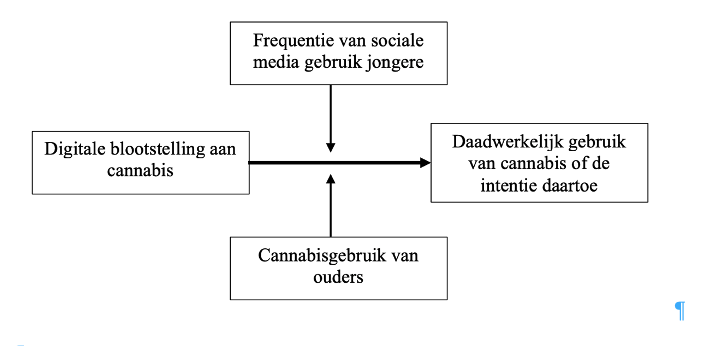
\includegraphics{images/Screenshot1.png}

}

\caption{Moderatieschema, hier alleen gebruik onderzocht}

\end{figure}

\hypertarget{methode}{%
\section{Methode}\label{methode}}

De dataverzameling voor deze studie vond plaats tussen 13 april 2023 en
9 mei 2023. Die onderzocht verschillende vormen van keuzegedrag onder
jongeren (zoals eetgewoontes, gebruik van sociale media, cannabis- en
alcoholgebruik) door middel van een vragenlijst in Qualtrics. Het
onderzoeksdesign is goedgekeurd door de ethiekcommissie (ERB) van de
Universiteit van Amsterdam (FMG-1280, 13-03-2023).

\hypertarget{steekproef}{%
\subsection{Steekproef}\label{steekproef}}

De vragenlijst is ingevuld door 166 respondenten, waarvan er 13 zijn
verwijderd uit de dataset vanwege het niet volledig invullen van de
vragenlijst. De overige participanten werden geïncludeerd in deze studie
(N = 153). De leeftijd van de participanten varieerde tussen de 16 en 24
jaar oud, met een gemiddelde leeftijd van 21.8 (SD = 2,18). Er deden 36
mannen (23.5\%) mee aan het onderzoek en 115 vrouwen (75.2\%). Op het
moment van afname volgden 106 participanten een opleiding (69.3\%) en
werkten er 32 (20.9\%). De meeste participanten volgde hoger onderwijs,
waarvan 42.5\% universitair (WO) en 19\% HBO. De meeste vaders van de
participanten volgde HBO als hoogst genoten opleiding (31.4\%), terwijl
de meeste moeders MBO als hoogst genoten opleidingsniveau hadden
(26.1\%).

\hypertarget{procedure}{%
\subsection{Procedure}\label{procedure}}

De participanten in deze studie werden grotendeels geworven via sociale
media. Daarnaast werden ook vrienden, familie en kennissen geworven voor
dit onderzoek. Een aanmeldvragenlijst werd via een URL-link gedeeld op
sociale media zoals Instagram, Facebook, WhatsApp en LinkedIn.
Potentiële deelnemers werden hierin gevraagd naar hun geboortedatum en
e-mailadres. Wanneer zij beide gegevens invulden konden ze de aanmelding
bevestigen, waarbij ze akkoord gingen dat ze binnen korte tijd een
vragenlijst zouden ontvangen op hun zojuist ingevulde e-mailadres.
Bovendien werd er vermeld dat onder de participanten (die hiermee
akkoord gingen) een cadeaubon van Bol.com ter waarde van 25 euro werd
verloot. Na het aanmelden via de korte vragenlijst ontvingen
participanten op korte termijn een digitale vragenlijst via Qualtrics.
Op de eerste pagina stond een korte uitleg over het onderzoek, waarna ze
werden verzocht de vragenlijst volledig en naar waarheid in te vullen.
Ook werd beschreven dat als zij de vragenlijst zouden starten, zij
akkoord gingen met deelname aan het onderzoek. Daarnaast werd duidelijk
gemaakt dat deelname volledig vrijwillig was en ze ten alle tijden
konden stoppen met het onderzoek. De vragenlijst die participanten
invulden vroeg hen naar daadwerkelijk cannabisgebruik, de intentie
daartoe en de online blootstelling daaraan. Naast deze vragen die
antwoord geven op de hoofdonderzoeksvragen, werden participanten ook
gevraagd naar verschillende vormen van keuzegedrag met betrekking tot
alcoholgebruik, eetgewoontes en risicogedrag in het algemeen. Deze
overige vragen werden toegevoegd om het doel van het onderzoek,
cannabisgebruik, te maskeren. Na het afsluiten van de dataverzameling
werd de dataset van Qualtrics geëxporteerd naar SPSS. Irrelevante
gegevens zoals taal, invultijd, IP-adres, start- en einddatum werden
verwijderd uit de variabelen. Vervolgens werden 5 variabelen
gehercodeerd, waarna 3 schalen gemaakt werden (zie paragraaf analyse).
In totaal werden 13 onvolledig ingevulde vragenlijsten (ofwel missings)
verwijderd uit de dataset. Van de afhankelijke variabelen werden
gestandaardiseerde scores gemaakt, zodat de scores op de verschillende
variabelen in verschillende analyses met elkaar vergeleken kunnen
worden.

\hypertarget{meetinstrumenten}{%
\subsection{Meetinstrumenten}\label{meetinstrumenten}}

De vragenlijst, 61 vragen bevattend, is door de onderzoekers opgesteld
en gebaseerd op betrouwbare vragenlijsten (Adamson et al., 2010; Defoe
et al., 2023; Martin et al., 2006; Vogel et al., 2021). Er werd gestart
met een aantal demografische vragen over leeftijd, geslacht, opleiding
en gezinssituatie. Vervolgens kregen participanten de opdracht om twee
minuten door hun Instagram te scrollen en deze sociale media posts te
bekijken. Hen werd vervolgens gevraagd hoeveel van de zojuist bekeken
posts pro- en anti-cannabis waren. De vragenlijst omvat daarnaast vragen
met betrekking tot de hoofdthema's van dit onderzoek, namelijk
cannabisgebruik, de intentie daartoe en de blootstelling aan cannabis
via sociale media. Tevens omvat de vragenlijst thema's gebaseerd op de
moderatoren van de onderzoekers zoals, sociaaleconomische status,
cannabisgebruik van ouders, vrienden of broers/zussen, het BIS/BAS
systeem, sensatiezoekend gedrag, impulsiviteit, motivatie voor
beloningen en sociale mediafrequentie. Zoals eerder benoemd, werden ook
overige thema's toegevoegd om het doel van het onderzoek te verbloemen.
Voor dit onderzoek zijn de volgende variabelen gebruikt:

\hypertarget{cannabisgebruik-1}{%
\subsubsection{Cannabisgebruik}\label{cannabisgebruik-1}}

Om het daadwerkelijke cannabisgebruik van de participanten te meten
werden de volgende vragen gebruikt: Gebruik je cannabis? (0 = Nee, ik
heb nooit cannabis gebruikt, 1 = Nee, op het moment niet, maar ik heb
wel eens cannabis gebruikt, 2 = Ja, minder dan één keer per maand, 3 =
Ja, tenminste één keer per maand, maar niet wekelijks, 4 = Ja, tenminste
één keer per week, maar niet iedere dag, 5 = Ja, iedere dag.); Hoe vaak
heb je in de afgelopen week cannabis gebruikt? (0 = Nooit, 1 = 1 of 2
maal, 2 = 3 of 4 maal, 3 = Dagelijks of bijna dagelijks); Hoe vaak heb
je cannabis gebruikt in de afgelopen 4 weken? (0 = Nooit, 1 = 1 tot 4
maal, 2 = 4 tot 7 maal, 3 = 7 tot 10 maal, 4 = 10 tot 14 maal, 5 = 14
tot 18 maal, 6 = Dagelijks of bijna dagelijks). Hogere scores op deze
items indiceren en hogere mate van daadwerkelijk cannabisgebruik. De
formulering van deze vragen en antwoordmogelijkheden is gebaseerd op de
CUDIT-R
{[}@adamson\_s\_j\_kay-lambkin\_f\_baker\_a\_l\_lewin\_t\_j\_thornton\_l\_kelly\_b\_\_improved\_nodate)
en een eerdere studie (Defoe et al., 2023). De schaal voor
cannabisgebruik behaalde een goede betrouwbaarheid (3 items; α = .807).

\hypertarget{online-blootstelling-aan-cannabis}{%
\subsubsection{Online blootstelling aan
cannabis}\label{online-blootstelling-aan-cannabis}}

Om de online blootstelling aan cannabis te meten bij participanten
werden de volgende vragen gebruikt: Hoe vaak kom je
cannabis-gerelateerde content op sociale media tegen? (0 = Nooit, 1 =
Minder vaak dan één keer per maand, 2 = 2 keer per maand, maandelijks, 3
= 1-3 keer per week, 4 = 4-6 keer per week, 5 = Dagelijks); Hoeveel
beroemdheden volg jij die cannabis gebruiken en dit laten zien op social
media? (0 = Ik volg geen beroemdheden die cannabis gebruiken op sociale
media, 1 = Ik volg een paar beroemdheden die cannabis gebruiken op
sociale media, 2 = Ik volg meer dan 10 beroemdheden die cannabis
gebruiken op sociale media, 3 = Ik volg meer dan 20 beroemdheden die
cannabis gebruiken op sociale media); Hoeveel vrienden volg jij die
cannabis gebruiken en dit laten zien op social media? (0 = Ik volg geen
vrienden die cannabis gebruiken op sociale media, 1 = Ik volg een paar
vrienden die cannabis gebruiken op sociale media, 2 = Ik volg meer dan
10 vrienden die cannabis gebruiken op sociale media, 3 = Ik volg meer
dan 20 vrienden die cannabis gebruiken op sociale media). Hogere scores
op deze items indiceren een hogere mate van online blootstelling aan
cannabis. De schaal online blootstelling aan cannabis behaalde een
betrouwbaarheid van α = .629 (3 items).

\hypertarget{sociale-media-frequentie}{%
\subsubsection{Sociale media
frequentie}\label{sociale-media-frequentie}}

Om de frequentie van het sociale media gebruik van participanten te
meten is gebruik gemaakt van de volgende vragen : Hoe vaak maak je
gebruik van sociale media, zoals Facebook, Instagram of Whatsapp? (0 =
Nooit, 1 = Maandelijks, 2 = Wekelijks, 3 = Dagelijks); Welke sociale
media gebruik je het meest? (0 = Instagram, 1 = Facebook, 2 = Twitter, 3
= Snapchat, 4= Reddit, 5 = Whatsapp, 6 = Anders, namelijk\ldots);
Hoeveel uur per dag gebruik je sociale media? (0 = Tussen de 0 en 3 uur,
1 = Tussen de 3 en 6 uur, 2 = Tussen de 6 en 9 uur, 3 = Tussen de 9 en
12 uur, 4 = Meer dan 12 uur). Hogere scores op deze items indiceren een
hogere mate van sociale media frequentie.

\hypertarget{cannabisgebruik-ouders}{%
\subsubsection{Cannabisgebruik ouders}\label{cannabisgebruik-ouders}}

Om het cannabisgebruik van ouders van participanten te meten is gebruik
gemaakt van de volgende vraag: Gebruikt tenminste één van je ouders
cannabis? (0 = Nee, deze persoon heeft nog nooit cannabis gebruikt, 1 =
Nee, op het moment niet, maar deze persoon heeft wel eens cannabis
gebruikt, 2 = Ja, minder dan één keer per maand, 3 = Ja, tenminste één
keer per maand, maar niet wekelijks, 4 = Ja, tenminste één keer per
week, maar niet per dag, 5 = Ja, iedere dag). Een hogere score op dit
item indiceert een hogere mate van cannabisgebruik door ouders. De
formulering van deze vraag en bijbehorende antwoordmogelijkheden is
gebaseerd op eerdere studies (Defoe et al., 2023; Martin et al., 2006).
Voor deze studie is deze variabele gedichotomiseerd. De ene groep zijn
ouders die nog nooit cannabis hebben gebruikt en de ander groep zijn de
ouders die wel eens tot en met iedere dat cannabis hebben gebruikt (deze
variabele is hier voor pedagogische redenen gedichotomiseerd)

\hypertarget{analyse}{%
\subsection{Analyse}\label{analyse}}

De dataverwerking en beschrijvende statistiek is uitgevoerd met behulp
van SPSS v.29 (IBM, Inc.), alle statistische analyses zijn uitgevoerd
met R (REF). Bij de analyses zijn de pakketten \texttt{haven} (om spss
bestanden binnen te halen), \texttt{tidyverse} (pakket voor
databewerking), \texttt{jtools} (om regressieanalyses goed in kaart te
brengen), \texttt{huxtable} (om tabel te tonen) en \texttt{interactions}
(om moderatie te visualiseren) gebruikt. Het reproduceerbare databestand
is hier in te zien (moderatie/rmd bestand) en hier is het pdf bestand
(moderatie/ ) van de analyse. Als eerste is (met SPSS) onderzocht of er
werd voldaan aan de assumpties voor een lineaire regressie, namelijk
lineairiteit, homoscedasticiteit, normaliteit en onafhankelijkheid
(Flatt \& Jacobs, 2019; Siero et al., 2009). De lineariteitsassumptie
vereist een rechte-lijn relatie tussen twee variabelen (Nimon, 2012). Na
het uitvoeren van een scatterplot in SPSS met cannabisgebruik als
afhankelijke variabele en online blootstelling als onafhankelijke
variabele blijkt dat deze dataset niet lineair is, waardoor niet wordt
voldaan aan deze assumptie. Daarnaast is er, op basis van de mediaan,
geen sprake van homoscedasticiteit, wat een constante spreiding tussen
de data vereist.\\
Daarentegen werd er wel voldaan aan het normaliteitsprincipe, daar de
waardes nauwelijks afweken van de diagonale lijn in het Q-Q diagram.
Tevens is de dataset redelijk onafhankelijk aangezien de respondenten
willekeurig gekozen zijn en deze elkaar niet beïnvloeden. Hierbij wordt
een kleine kanttekening gemaakt, omdat alle participanten uit de
vrienden-, familie- en kennissenkring van de onderzoekers komen.
Aangezien niet wordt voldaan aan de lineairiteit- en
homoscedasticiteitsassumptie zullen de resultaten voorzichtig
geïnterpreteerd moeten worden. Een regressieanalyse is toch uitgevoerd,
mede omdat heteroscedasticiteit (ofwel het niet aanwezig zijn van
homoscedasticiteit) maar een klein effect heeft op significantietesten
(Osbourne \& Waters, 2002). Vervolgens is er met R gewerkt. Eerst is een
enkelvoudige regressie uitgevoerd om een eventuele relatie tussen een
onafhankelijke en afhankelijke variabele te onderzoeken (Cohen et al.,
2014). Deze enkelvoudige regressie zal in deze studie uitgevoerd worden
om cannabisgebruik te voorspellen op basis van blootstelling aan
cannabis op sociale media. Vervolgens zal aan de hand van meervoudige
regressie de voorspelbaarheid van cannabisgebruik geanalyseerd worden op
basis van online blootstelling en frequentie van sociale media gebruik
en vervolgens cannabisgebruik van ouders of frequentie van sociale media
gebruik. Het doel van deze meervoudige regressie is analyseren welke
combinatie van onafhankelijke variabelen de meeste invloed heeft op de
afhankelijke variabele (Cohen et al., 2014). Als laatste zullen
moderatieanalyses (Hayes, 2013) uitgevoerd worden, om cannabisgebruik te
voorspellen op basis van online blootstelling en waarbij cannabisgebruik
van ouders of sociale media frequentie de relatie tussen
cannabisgebruik/intentie en online blootstelling modereert. Een
moderatieanalyse wordt uitgevoerd om te onderzoeken of de relatie tussen
een afhankelijke en onafhankelijke variabele verandert door middel van
de derde variabele, de moderator (Baron \& Kenny, 1986).

\hypertarget{resultaten}{%
\section{Resultaten}\label{resultaten}}

\hypertarget{beschrijvende-statistiek}{%
\subsection{Beschrijvende statistiek}\label{beschrijvende-statistiek}}

De beschrijvende statistieken werden berekend om inzicht te krijgen in
de kenmerken van de steekproef. Van alle participanten heeft 43.1\% nog
nooit cannabis gebruikt (\(M\) = .74, \(SD\) = .946). Daarentegen geeft
60.1\% aan ooit wel eens te hebben gebruikt, waarvan 11.1\% momenteel
ook nog consumeert. In de afgelopen vier weken heeft 8.6\% van de
participanten cannabis gebruikt (\(M\) = .16, \(SD\) = .000) en 4.7\% in
de afgelopen week (\(M\) = .07, \(SD\) = .000). Volgend jaar verwacht
17.6\% van de jongeren (nog steeds) cannabis te gebruiken (\(M\) = 1.21,
\(SD\) = 1.807). Daarnaast geeft 27.5\% aan minder dan één keer per
maand cannabis-gerelateerde content tegen te komen op sociale media,
waarbij 6.6\% wekelijks aan deze content wordt blootgesteld (\(M\) =
.75, \(SD\) = 1.045). Wat betreft het volgen van accounts op sociale
media, geeft 22.9\% aan dat zij een paar beroemdheden volgen die
cannabis gebruiken, terwijl 63.4\% geen beroemdheden volgt die die
content plaatsen (\(M\) = .32, \(SD\) = .556). 29.4\% van de
participanten volgt een paar vrienden die cannabis gebruiken en dit
laten zien op sociale media (\(M\) = .39, \(SD\) = .586). Tevens gaven
alle participanten aan sociale media dagelijks te gebruiken (\(M\) =
3.0, \(SD\) = .000), waarvan de meeste tussen de 3 en 6 uur per dag
(49.0\%; \(M\) = .72, \(SD\) = .650). De dagelijks meest gebruikte
platforms waren WhatsApp (42.5\%) en Instagram (28.1\%). Verder gaf
26.8\% van de participanten aan dat tenminste één van zijn/haar ouders
op dit moment geen cannabis gebruikt, maar deze persoon het wel eens
heeft geconsumeerd (\(M\) = .36, \(SD\) = .647). Daarnaast gebruikt
tenminste één ouder van 0.7\% van de participanten minder dan één keer
per maand cannabis, terwijl 1.3\% tenminste één keer per week gebruikt.

\hypertarget{digitale-blootstelling-aan-cannabis-en-het-daadwerkelijke-gebruik-onder-jongeren}{%
\subsection{Digitale blootstelling aan cannabis en het daadwerkelijke
gebruik onder
jongeren}\label{digitale-blootstelling-aan-cannabis-en-het-daadwerkelijke-gebruik-onder-jongeren}}

Eerst wordt een enkelvoudige regressie (model 1) uitgevoerd om
cannabisgebruik te voorspellen op basis van blootstelling aan cannabis
op sociale media. De resultaten van deze analyse laten zien dat online
blootstelling aan cannabis een significante voorspeller is voor
cannabisgebruik (\(\beta\) = .33, \(p\) \textless{} .001). Dit geeft aan
dat er een verband bestaat tussen digitale blootstelling aan cannabis en
daadwerkelijk cannabisgebruik. De regressievergelijking was significant,
\(F(1, 134) = 14.56, p <.001\) en online blootstelling verklaarde 10\%
van de variantie in cannabisgebruik (\(R^2 = .10\)). Deze verklaarde
variantie geeft aan dat de individuele verschillen in cannabisgebruik
voor een minimaal deel zijn terug te voeren aan de blootstelling aan
cannabis op sociale media. Tevens blijkt dus dat er een kleine
significante relatie bestaat tussen online blootstelling aan cannabis en
daadwerkelijk cannabisgebruik. Met andere woorden: iemand die vaker
wordt blootgesteld aan cannabis op sociale media over het algemeen vaker
cannabis gebruikt in de werkelijkheid.

\hypertarget{sociale-media-frequentie-als-moderator-bij-daadwerkelijk-cannabisgebruik}{%
\subsubsection{Sociale media frequentie als moderator bij daadwerkelijk
cannabisgebruik}\label{sociale-media-frequentie-als-moderator-bij-daadwerkelijk-cannabisgebruik}}

\begin{figure}

{\centering 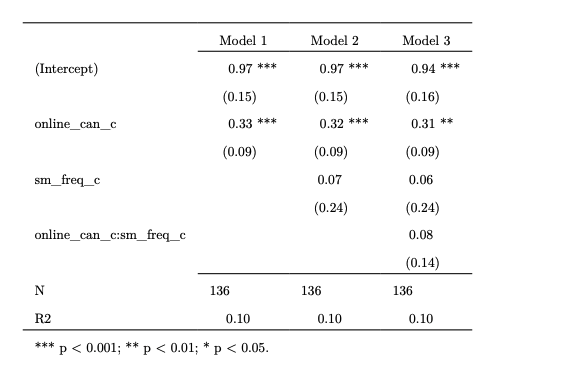
\includegraphics{images/Screenshot1a.png}

}

\caption{Modellen naast elkaar gezet}

\end{figure}

Vervolgens wordt een meervoudige regressieanalyse (model 2) uitgevoerd
om de voorspelbaarheid van cannabisgebruik te analyseren op basis van
online blootstelling en beide moderatoren, te beginnen met de frequentie
van sociale media gebruik. De resultaten van deze analyse laten een
statistisch significant model zien: \(F(2,133) = 7.27, p = .001\). Het
model verklaart 10\% van de variantie van cannabisgebruik
(\(R^2 = .10\)). Online blootstelling
(\(\beta = 0.32, t = 3.56, p <.001)\) is een significante voorspeller
van cannabisgebruik bij jongeren, maar de frequentie van sociale media
gebruik is dit niet (\(\beta = 0.07, t = .030, p = .76\)). Om te
onderzoeken of de frequentie van het sociale media gebruik van jongeren
dan een modererende rol speelt op de relatie tussen online blootstelling
en cannabisgebruik werd een moderatoranalyse (model 3) uitgevoerd. De
resultaten tonen een significant model met de voorspellers online
blootstelling aan cannabis, sociale media frequentie en het
interactie-effect, \(F(3, 132) = 4.94, p = .003, R^2 = .10\). Dit model
verklaart dus 10\% van de variantie van cannabisgebruik. Echter toonden
de resultaten geen significant interactie-effect tussen online
blootstelling aan cannabis en de frequentie van sociale media gebruik
(\(\beta = .06, t = 0.23, p = .82)\). In tabel 1 zijn bovenstaande drie
modellen naast elkaar gezet. Hier is te zien dat de meervoudige
regressie (model 2) en de moderatieanalyse (model 3) geen significantie
opleveren voor de variabelen die zijn toegevoegd. De frequentie van
sociale media gebruik modereert dus niet in de relatie tussen online
blootstelling aan cannabis en daadwerkelijk cannabisgebruik. In Figuur 2
staan de modellen naast elkaar.

Dat er geen interactie-effect te zien is, maakt Figuur 3 duidelijk.

\begin{figure}

{\centering 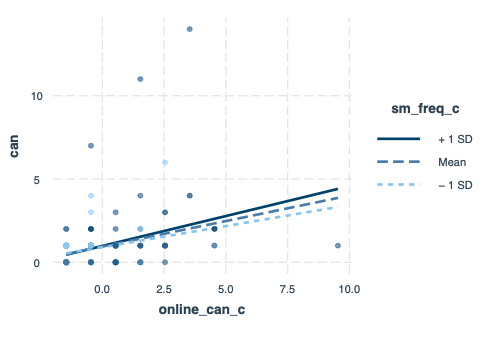
\includegraphics{images/Screenshot2.png}

}

\caption{Visualisatie van moderatieeffect}

\end{figure}

\hypertarget{ouderlijk-cannabisgebruik-als-moderator-bij-daadwerkelijk-cannabisgebruik}{%
\subsubsection{Ouderlijk cannabisgebruik als moderator bij daadwerkelijk
cannabisgebruik}\label{ouderlijk-cannabisgebruik-als-moderator-bij-daadwerkelijk-cannabisgebruik}}

\begin{figure}

{\centering 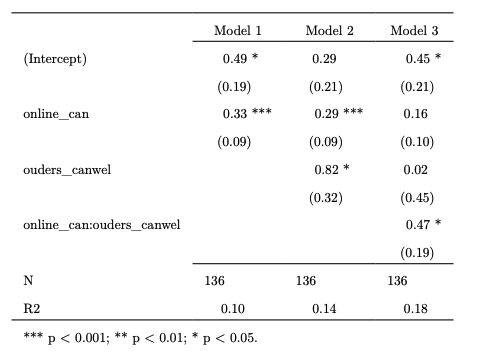
\includegraphics{images/Screenshot3.png}

}

\caption{Modellen naast elkaar gezet}

\end{figure}

De resultaten van de enkelvoudige regressieanalyse tussen
cannabisgebruik van jongeren en online blootstelling cannabisgebruik
zagen we hierboven. Nu voegen we extra (dichotome) variabele (ouderlijk
cannabisgebruik, wel of nooit gebruik) toe in de meervoudige
regressieanalyse. Op basis van digitale blootstelling en het ouderlijk
cannabisgebruik wordt hier de voorspelbaarheid van cannabisgebruik bij
jongeren geanalyseerd middels een meervoudige regressieanalyse. Uit deze
resultaten blijkt ook een significant model:
\(F(2,133) = 10.91, p < .001\). Dit model blijkt 14\% van de variantie
van cannabisgebruik te verklaren (\(R^2 = .14\)). Online blootstelling
(\(\beta = .29, t = 3,41 p <.001\)) en het ouderlijk cannabisgebruik
(\(\beta = .82, t = .140, p =.01\)) blijken beide significante
voorspellers voor het cannabisgebruik van jongeren. Vervolgens wordt een
moderatieanalyse gedaan om de moderende rol van de variabele ouderlijk
cannabisgebruik te onderzoeken. De resultaten laten een significant
model zien met voorspellers online blootstelling aan cannabis, ouderlijk
cannabisgebruik en het interactie-effect:
\(F(3, 132) = 9.63, p < .001, R^2 = .18\). Dit model verklaart 18\% van
de variantie in cannabisgebruik. Bovendien toonden de resultaten hiervan
wel een statistisch significant interactie-effect tussen online
blootstelling en cannabisgebruik van ouders
(\(β = .47, t(132) = 2.49, p = .01\)). Dit suggereert dat het ouderlijk
cannabisgebruik de relatie tussen online blootstelling aan cannabis en
daadwerkelijk cannabisgebruik beïnvloed. In tabel 2 zijn de drie
modellen wat betreft de relatie tussen online blootstelling en
daadwerkelijk cannabisgebruik met moderator ouderlijk cannabisgebruik
naast elkaar gezet. Hier is te zien dat de moderatieanalyse (model 3)
duidelijk het sterkste is. Het ouderlijk cannabisgebruik modereert dus
wel in de relatie tussen online blootstelling aan cannabis en
daadwerkelijk cannabisgebruik. Figuur 4 zet de modellen op rij.

Het gevonden interactie-effect is in Figuur 5 duidelijk te zien.

\begin{figure}

{\centering 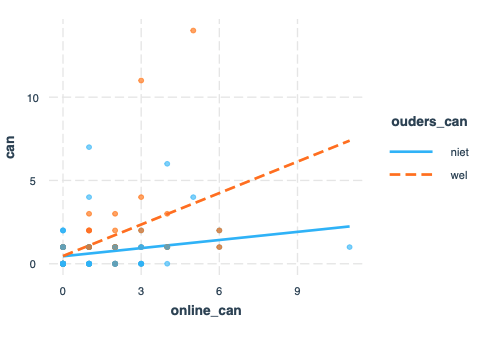
\includegraphics{images/Screenshot4.png}

}

\caption{Visualisatie van het interactieeffect}

\end{figure}

\hypertarget{discussie}{%
\section{Discussie}\label{discussie}}

Op basis van de eerdergenoemde zorgelijke cijfers rondom cannabisgebruik
en sociale media en daarbij de bijzonder kwetsbare leeftijdsgroep is in
deze studie onderzoek gedaan naar de invloed van blootstelling via
sociale media om meer inzicht te krijgen in mogelijke verklaringen voor
het toenemende drugsgebruik onder jongvolwassenen. Aangezien
cannabisgebruik in de ontwikkelingsfase van jongeren schadelijke
gevolgen kan hebben voor zowel de geestelijke gezondheid, als werk en
opleiding, lijkt het achterhalen van de oorzaak van groot belang
(Fergusson \& Boden, 2008; Lee et al., 2015). Het doel van deze huidige
studie was dan ook om te bepalen of online blootstelling aan cannabis
het daadwerkelijke cannabisgebruik of de intentie tot cannabisgebruik
van jongvolwassenen kan voorspellen.

\hypertarget{digitale-blootstelling-aan-cannabis-en-het-daadwerkelijke-gebruik-onder-jongeren-1}{%
\subsection{Digitale blootstelling aan cannabis en het daadwerkelijke
gebruik onder
jongeren}\label{digitale-blootstelling-aan-cannabis-en-het-daadwerkelijke-gebruik-onder-jongeren-1}}

De hoofdvraag `In hoeverre bestaat er een relatie tussen digitale
blootstelling aan cannabis en het daadwerkelijk gebruik van cannabis
onder jongeren van 16 tot en met 24 jaar?' is onderzocht aan de hand van
een enkelvoudige regressieanalyse. Op basis van het DNERM (Defoe, 2021)
werd verwacht dat jongeren die digitaal vaker werden blootgesteld aan
cannabis in de realiteit vaker cannabis zouden gebruiken. Uit de
enkelvoudige regressieanalyse bleek een klein positief significant
effect, wat wil zeggen dat een toename in de digitale blootstelling aan
cannabis gepaard gaat met een lichte toename in cannabisgebruik. Deze
bevinding is in lijn met de gevormde hypothese, aangezien (digitale)
blootstelling aan cannabis kan leiden tot nieuwsgierigheid of verlangen
(Defoe, 2021). Deze attitudes onderhouden een directe relatie met
gedrag, waardoor iemand die online meer wordt blootgesteld aan cannabis
inderdaad ook iets vaker daadwerkelijk cannabis gebruikt. Tevens is de
modererende rol van de frequentie van het sociale media gebruik van
jongeren op de veronderstelde relatie uit de hoofdvraag onderzocht.
Aangezien deze factor nog nauwelijks onderzocht is als mogelijk
moderatie-effect is de hypothese gebaseerd op andere onderzoeken.
Verwacht werd dat de relatie tussen online blootstelling aan cannabis en
het daadwerkelijke gebruik versterkt zou worden wanneer jongeren een
hogere gebruiksfrequentie hadden. Deze hypothese werd gebaseerd op de
PBT en de veronderstelling dat jongeren die niet actief zijn op sociale
media minder middelen gebruiken dan jongeren die wel actief zijn
(Boniel-Nissim et al., 2022; Westgate \& Holliday, 2016; Jessor \&
Jessor, 1977). Uit de resultaten van de moderatoranalyse bleek geen
significant interactie-effect, wat wil zeggen dat een hogere of lagere
frequentie van sociale media gebruik geen invloed heeft op de relatie
tussen online blootstelling en het daadwerkelijk cannabisgebruik. Uit de
literatuur blijkt (nog) geen mogelijke verklaring (mede omdat er geen
eerder onderzoek is gedaan naar dit moderatie-effect). Een mogelijke
verklaring zou het algoritme van sociale media kunnen zijn, aangezien
deze platforms precies onthouden wat men leuk vindt, zodat een
gepersonaliseerd aanbod wordt gepresenteerd. Hierin geldt een
zelfversterkend effect dat ook wel de filterbubbel wordt genoemd:
wanneer men bepaalde dingen interessant vindt, zullen deze vaker
aangeboden worden, waarmee andere berichten buiten het gezichtsveld van
diegene vallen (Pariser, 2011). Een jongere die bijvoorbeeld nog nooit
cannabis heeft opgezocht op sociale media en geen vrienden of
beroemdheden volgt die cannabis gerelateerde content plaatsen, zal geen
spontane berichten aangeboden krijgen (onafhankelijk van hoe vaak
diegene sociale media ook gebruikt). Naast de factor sociale media
frequentie is ook de modererende rol van de variabele ouderlijk
cannabisgebruik onderzocht. Ook deze variabele is nauwelijks onderzocht,
waardoor geen moderatie-effect gevonden is in de huidige literatuur. Op
basis van de attitude van ouders die gebruiken ten opzichte van
cannabisgebruik en de verminderde monitoring en ouder-kindrelatie werd
verwacht dat, hoe vaker ouders cannabis gebruiken, hoe sterker de
relatie tussen online blootstelling aan cannabis en het daadwerkelijke
gebruik (Rusby et al., 2018; Vaala \& Bleakley, 2015; Cho \& Cheon,
2005). Uit de resultaten van de moderatoranalyse bleek een significant
interactie-effect. Met andere woorden ouderlijk cannabisgebruik
beïnvloedt de relatie tussen online blootstelling aan cannabis en het
daadwerkelijke gebruik. Hierbij bleek dat wanneer het ouderlijk
cannabisgebruik gemiddeld of hoog was, de relatie tussen digitale
blootstelling en gebruik versterkt werd. Deze bevinding sluit aan op de
verwachtingen, waarbij de verklaring zich mogelijk vindt in de attitude
van ouders richting cannabis, waarbij jongeren sneller online hiermee in
`aanraking' komen wanneer ouders acceptatie uitstralen ten opzichte van
de drug (Rusby et al., 2018).

\hypertarget{limitaties-en-sterktes}{%
\subsection{Limitaties en sterktes}\label{limitaties-en-sterktes}}

Zoals bij vrijwel ieder onderzoek waren er ook bij deze studie
limitaties. Ten eerste kan de samenstelling van de steekproef invloed
hebben gehad op de resultaten, aangezien deze zijn verkregen via sociale
media, vrienden/familie en kenniskringen in een redelijk korte periode
van dataverzameling. De onderzoekers zijn allen hoogopgeleid, wat
suggereert dat hun vrienden- en kenniskring (via sociale media) ook
hoogopgeleid zijn, aangezien mensen vaker contact hebben met mensen met
een vergelijkbaar opleidingsniveau (Völker et al., 2014). Mogelijk heeft
dit gezorgd voor een vertekend beeld en is deze steekproef niet
generaliseerbaar voor de algehele populatie. Ten tweede is de
vragenlijst die is ingevuld door de respondenten zelfstandig door de
onderzoekers ontwikkeld vanuit verschillende andere vragenlijsten. De
vraagstellingen en antwoordmogelijkheden waren zo veel als mogelijk
identiek aan eerdere theorie, hierbij is de formulering passend gemaakt
voor deze studie naar cannabisgebruik. Mogelijk heeft dit invloed gehad
op de betrouwbaarheid van de vragenlijst. Daarnaast omvatten de
onderzochten constructen vaak maar enkele items, wat de betrouwbaarheid
van de vragenlijst mogelijk ook niet ten goede komt. Ten derde is
cannabisgebruik als onderwerp erg kwetsbaar, zeker bij jongeren die nog
in zekere zin afhankelijk zijn of verantwoording afleggen aan ouders.
Mogelijk heeft niet iedere respondent rond dit onderwerp naar alle
eerlijkheid de vragenlijst ingevuld en is er sprake van sociaal
wenselijke antwoorden. Deze neiging onder participanten om hun
antwoorden sociaal wenselijk te maken heeft invloed op de validiteit van
onderzoeksgegevens (Tijmstra \& Brinkman-Engels, 1978). Ondanks deze
beperkingen heeft deze studie wel degelijk bijgedragen aan het vergroten
van de kennis over een relatief onbekende directe relatie tussen
blootstelling aan cannabis op sociale media en het daadwerkelijke
gebruik of de intentie daartoe. Eerder onderzoek heeft zich hier tot nu
toe nog nauwelijks specifiek op gericht, waardoor in dat opzicht dit
onderzoek alleen al vernieuwend is. Daarnaast heeft het onderzoek zich
grotendeels gebaseerd op een nieuwe theorie, DNERM. Nieuw onderzoek is
hier toegevoegd aan een theoretisch kader dat nog nauwelijks is gebruikt
in andere studies. Hierbij lijkt het van belang te veronderstellen dat
gedrag wordt beïnvloed door verschillende factoren, waardoor men zich
ook niet maar op één aspect moet richten in onderzoek.

\hypertarget{implicaties}{%
\subsection{Implicaties}\label{implicaties}}

In toekomstig onderzoek zou het ten eerste interessant zijn om voor het
afnemen van de vragenlijst deze uitgebreid te onderleggen aan
validiteitsonderzoek en waar nodig aan te passen om de betrouwbaarheid
te vergroten. Op deze manier kunnen hardere conclusies getrokken worden
uit de resultaten van het bijbehorende onderzoek. Daarnaast zou het
analyseren van meerdere moderatoren binnen de bestaande relatie tussen
online blootstelling en daadwerkelijk gebruik of de intentie daartoe
interessant zijn, zodat preventieve interventie gericht ingezet kan
worden. De toename van het sociale media gebruik is momenteel een trend
die niet makkelijk lijkt te doorbreken. Daarentegen lijkt die trend van
cannabisgebruik, met op het eerste oog een grotere negatieve impact,
directer te beïnvloeden wanneer specifiek op bepaalde factoren ingezet
kan worden. Een implicatie voor de praktijk wordt vooral gebaseerd op de
bevindingen rondom de modererende rol van het ouderlijk cannabisgebruik.
Het lijkt hier van belang in te zetten op de attitudes van ouders ten
opzichte van het cannabisgebruik, aangezien deze een waarschijnlijke
verklaring vormen voor het versterkende effect op de relatie tussen
digitale blootstelling en gebruik/intentie. Het advies is om tijdens
ouderschapstrainingen en bijeenkomsten waar ouders informatie verkrijgen
over het ouderschap in te zetten op het vergroten van het besef wat
betreft de invloed van hun attitude op hun kind. Hierbij dient rekening
gehouden te worden met de adolescentieperiode als belangrijkste fase.
Een mogelijke optie zouden bijeenkomsten voor ouders kunnen zijn bij
aanvang van de middelbare school.

\hypertarget{conclusie}{%
\subsection{Conclusie}\label{conclusie}}

In deze studie is gezocht naar een antwoord op de vraag: `In hoeverre
bestaat er een relatie tussen digitale blootstelling aan cannabis en het
daadwerkelijk gebruik onder jongeren van 16 tot en met 24 jaar?'. Ter
beantwoording is cross-sectioneel onderzoek uitgevoerd naar
cannabisgebruik en het effect van sociale media aan de hand van data
verkregen uit een vragenlijst. Uit de resultaten blijkt dat, in lijn met
DNERM, TPB en eerder onderzoek, hoe vaker de jongere online wordt
blootgesteld aan cannabis, hoe vaker daadwerkelijk cannabis gebruikt
wordt. Ook blijkt dat de frequentie van het sociale media gebruik van de
jongere geen modererende rol speelt in deze relatie. Het cannabisgebruik
van ouders heeft daarentegen wel een moderatie-effect binnen dit
verband. Een gemiddelde of hoge mate van ouderlijk cannabisgebruik
versterkt de relatie tussen online blootstelling en daadwerkelijk
gebruik. Al met al benadrukken deze bevindingen de invloed van sociale
media op het cannabisgebruik van jongvolwassenen, waardoor het van
belang is bewustzijn (onder ouders) te vergroten en preventieve
maatregelen te nemen om de potentiële schadelijke gevolgen van het
cannabisgebruik en de online omgeving aan te pakken.

\hypertarget{literatuur}{%
\subsection{Literatuur}\label{literatuur}}

Adamson, S. J., Kay-Lambkin, F., Baker, A. L., Lewin, T. J., Thornton,
L., Kelly, B., \& Sellman, J. D. (2010). An improved brief measure of
cannabis misuse: The Cannabis Use Disorders Identification Test-Revised
(CUDIT-R). \emph{Drug and Alcohol Dependence}, 110(1--2), 137--143.
https://doi.org/10.1016/j.drugalcdep.2010.02.017

Ajzen, I. (1991). The theory of planned behavior. \emph{Organizational
Behavior and Human Decision Processes, 50(2)}, 179--211.
https://doi.org/10.1016/0749-5978(91)90020-t

Amiet, D., Youssef, G. J., Hagg, L. J., Lorenzetti, V., Parkes, L.,
Solowij, N., \& Yücel, M. (2020). Young Adults With Higher Motives and
Expectancies of Regular Cannabis Use Show Poorer Psychosocial
Functioning. \emph{Frontiers in Psychiatry, 11}.
https://doi.org/10.3389/fpsyt.2020.599365

Baron, R. M., \& Kenny, D. A. (1986). The moderator--mediator variable
distinction in social psychological research: Conceptual, strategic, and
statistical considerations. \emph{Journal of Personality and Social
Psychology, 51(6)}, 1173--1182.
https://doi.org/10.1037/0022-3514.51.6.1173

Bayer, J. B., Triệu, P., \& Ellison, N. B. (2020). Social Media
Elements, Ecologies, and Effects. \emph{Annual Review of Psychology,
71(1)}, 471--497. https://doi.org/10.1146/annurev-psych-010419-050944

Bechtold, J., Simpson, T. M., White, H. R., \& Pardini, D. A. (2015).
Chronic adolescent marijuana use as a risk factor for physical and
mental health problems in young adult men. \emph{Psychology of Addictive
Behaviors, 29(3)}, 552--563. https://doi.org/10.1037/adb0000103

Berryman, C., Ferguson, C. J., \& Negy, C. (2018). Social Media Use and
Mental Health among Young Adults. \emph{Psychiatric Quarterly, 89(2)},
307--314. https://doi.org/10.1007/s11126-017-9535-6

Boniel-Nissim, M., Van Den Eijnden, R. J. J. M., Furstova, J., Marino,
C., Lahti, H., Inchley, J., Šmigelskas, K., Vieno, A., \& Badura, P.
(2022). International perspectives on social media use among
adolescents: Implications for mental and social well-being and substance
use. \emph{Computers in Human Behavior, 129}, 107144.
https://doi.org/10.1016/j.chb.2021.107144

Borges, G., Bagge, C. L., \& Orozco, R. (2016). A literature review and
meta-analyses of cannabis use and suicidality. \emph{Journal of
Affective Disorders, 195}, 63--74.
https://doi.org/10.1016/j.jad.2016.02.007

Branley-Bell, D., \& Covey, J. (2017). Is exposure to online content
depicting risky behavior related to viewers' own risky behavior offline?
\emph{Computers in Human Behavior, 75}, 283--287.
https://doi.org/10.1016/j.chb.2017.05.023

Brook, J. S., Zhang, C., Koppel, J., \& Brook, D. W. (2008). Pathways
from Earlier Marijuana Use in the Familial and Non-Familial Environments
to Self-Marijuana Use in the Fourth Decade of Life. \emph{American
Journal on Addictions, 17(6)}, 497--503.
https://doi.org/10.1080/10550490802408373

Centraal Bureau voor de Statistiek. (2020). \emph{Nederland in cijfers}.
https://longreads.cbs.nl/nederland-in-cijfers-2020/wie-gebruikt-het-vaakst-sociale-
media/

Cho, C., \& Cheon, H. J. (2005). Children's Exposure to Negative
Internet Content: Effects of Family Context. \emph{Journal of
Broadcasting \& Electronic Media, 49(4)}, 488--509.
https://doi.org/10.1207/s15506878jobem4904\_8

Cohen, J., Cohen, P., West, S. C., \& Aiken, L. S. (2014). Applied
Multiple Regression/Correlation Analysis for the Behavioral Sciences. In
\emph{Psychology Press eBooks}. https://doi.org/10.4324/9781410606266

Crone, E. A., \& Dahl, R. E. (2012). Understanding adolescence as a
period of social--affective engagement and goal flexibility.
\emph{Nature Reviews Neuroscience, 13(9)}, 636--650.
https://doi.org/10.1038/nrn3313

Defoe, I. N. (2021). Towards a hybrid criminological and psychological
model of risk behavior: The developmental neuro-ecological risk-taking
model (DNERM). \emph{Developmental Review, 62, 100995}.
https://doi.org/10.1016/j.dr.2021.100995

Defoe, I. N., Dubas, J. S., Figner, B., \& Van Aken, M. a. G. (2015). A
meta-analysis on age differences in risky decision making: Adolescents
versus children and adults. \emph{Psychological Bulletin, 141(1)},
48--84. https://doi.org/10.1037/a0038088

Defoe, I. N., Dubas, J. S., \& Van Aken, M. A. G. (2023). A
cross‐national study on adolescent substance use: Intentions, peer
substance use, and parent‐adolescent communication. \emph{Journal of
Research on Adolescence, 33(2)}, 1--15.
https://doi.org/10.1111/jora.12832

Europees Waarnemingscentrum voor drugs en drugsverslaving. (2019).
\emph{Europees Drugsrapport 2019: Trends en ontwikkelingen}. Bureau voor
publicaties van de Europese Unie.
https://www.emcdda.europa.eu/system/files/publications/11364/20191724\_TDAT190
01NLN\_PDF.pdf

Fergusson, D. M., \& Boden, J. M. (2008). Cannabis use and later life
outcomes. \emph{Addiction, 103(6)}, 969--976.
https://doi.org/10.1111/j.1360-0443.2008.02221.x

Flatt, C., \& Jacobs, R. L. (2019). Principle Assumptions of Regression
Analysis: Testing, Techniques, and Statistical Reporting of Imperfect
Data Sets. \emph{Advances in Developing Human Resources, 21(4)},
484--502. https://doi.org/10.1177/1523422319869915

Gobbi, G., Atkin, T., Zytynski, T., Wang, S., Askari, S., Boruff, J.,
Ware, M. A., Marmorstein, N. R., Cipriani, A., Dendukuri, N., \& Mayo,
N. E. (2019). Association of Cannabis Use in Adolescence and Risk of
Depression, Anxiety, and Suicidality in Young Adulthood. \emph{JAMA
Psychiatry, 76(4)}, 426.
https://doi.org/10.1001/jamapsychiatry.2018.4500

Hall, W., \& Degenhardt, L. (2009). Adverse health effects of
non-medical cannabis use. \emph{The Lancet, 374(9698)}, 1383--1391.
https://doi.org/10.1016/s0140-6736(09)61037-0

Hall, W., \& Degenhardt, L. (2014). The adverse health effects of
chronic cannabis use. \emph{Drug Testing and Analysis, 6(1--2)}, 39--45.
https://doi.org/10.1002/dta.1506

Hall, W., Leung, J., \& Lynskey, M. T. (2020). The effects of cannabis
use on the development of adolescents and young adults. \emph{Annual
Review of Developmental Psychology, 2(1)}, 461--483.
https://doi.org/10.1146/annurev-devpsych-040320-084904

Hayes, A. F. (2013). \emph{Introduction to Mediation, Moderation, and
Conditional Process Analysis: A Regression-Based Approach}.
https://ci.nii.ac.jp/ncid/BB1323391X

Hernández-Serrano, O., Gras, M. E., Gacto, M., Brugarola, A., \&
Font-Mayolas, S. (2021). Family Climate and Intention to Use Cannabis as
Predictors of Cannabis Use and Cannabis-Related Problems among Young
University Students. \emph{\&International Journal of Environmental
Research and Public Health, 18(17)}, 9308.
https://doi.org/10.3390/ijerph18179308

Jalilian, F., Mirzaei-Alavijeh, M., Ahmadpanah, M., Mostafaei, S.,
Kargar, M., Pirouzeh, R., Bahmani, D. S., \& Brand, S. (2020). Extension
of the Theory of Planned Behavior (TPB) to Predict Patterns of Marijuana
Use among Young Iranian Adults. \emph{International Journal of
Environmental Research and Public Health, 17(6)}, 1981.
https://doi.org/10.3390/ijerph17061981

Jessor, R., \& Jessor, S. L. (1977). Problem Behavior and Psychosocial
Development: A Longitudinal Study of Youth. Academic Press. Lee, J. P.,
Brook, J. S., Finch, S. J., \& Brook, D. W. (2015). Trajectories of
marijuana use from adolescence to adulthood predicting unemployment in
the mid 30s. \emph{American Journal on Addictions, 24(5)}, 452--459.
https://doi.org/10.1111/ajad.12240

Martin, G. S., Copeland, J., Gates, P., \& Gilmour, S. (2006). The
Severity of Dependence Scale (SDS) in an adolescent population of
cannabis users: Reliability, validity and diagnostic cut-off. \emph{Drug
and Alcohol Dependence, 83(1)}, 90--93.
https://doi.org/10.1016/j.drugalcdep.2005.10.014

Miller, S. D., Siegel, J. B., Hohman, Z. P., \& Crano, W. D. (2013).
Factors mediating the association of the recency of parent's marijuana
use and their adolescent children's subsequent initiation.
\emph{Psychology of Addictive Behaviors, 27(3)}, 848--853.
https://doi.org/10.1037/a0032201

Nimon, K. (2012). Statistical Assumptions of Substantive Analyses Across
the General Linear Model: A Mini-Review. \emph{Frontiers in Psychology,
3}. https://doi.org/10.3389/fpsyg.2012.00322

Osbourne, J. W., \& Waters, E. M. (2002). Four Assumptions of Multiple
Regression That Researchers Should Always Test. \emph{Practical
Assessment, Research and Evaluation, 8(2)}, 2.
https://doi.org/10.7275/r222-hv23

Pariser, E. (2011). \emph{The Filter Bubble: What the Internet Is Hiding
from You}. https://dl.acm.org/citation.cfm?id=2029079

Rusby, J. C., Light, J. C., Crowley, R., \& Westling, E. (2018).
Influence of parent--youth relationship, parental monitoring, and parent
substance use on adolescent substance use onset. \emph{Journal of Family
Psychology, 32(3)}, 310--320. https://doi.org/10.1037/fam0000350

Schilling, S., Melzer, R., \& McCabe, P. F. (2020). Cannabis sativa.
\emph{Current Biology, 30}, R8-- R9.
https://www.cell.com/current-biology/pdf/S0960-9822(19)31379-X.pdf

Siero, F. W., Huisman, M., \& Kiers, H. A. (2009). \emph{Assumpties en
generalisaties}. In Bohn Stafleu van Loghum eBooks (pp.~47--75).
https://doi.org/10.1007/978-90-313-7359-8\_3

Starri, M. (2022, February 1). \emph{Report Digital 2020: i dati global.
We Are Social Italy}.
https://wearesocial.com/it/blog/2020/01/report-digital-2020-i-dati-global/

Steinberg, L. (2007). Risk Taking in Adolescence. \emph{Current
Directions in Psychological Science, 16(2)}, 55--59.
https://doi.org/10.1111/j.1467-8721.2007.00475.x

Tijmstra, T., \& Brinkman-Engels, M. (1978). Sociale wenselijkheid als
validiteitsprobleem. \emph{Mens En Maatschappij, 53(2)}, 196--208.
https://rjh.ub.rug.nl/MenM/article/download/13195/10695

Vaala, S. E., \& Bleakley, A. (2015). Monitoring, Mediating, and
Modeling: Parental Influence on Adolescent Computer and Internet Use in
the United States. \emph{Journal of Children and Media, 9(1)}, 40--57.
https://doi.org/10.1080/17482798.2015.997103

Valkenburg, P. M. (2021). Social media use and well-being: What we know
and what we need to know. \emph{Current Opinion in Psychology, 45},
101294. https://doi.org/10.1016/j.copsyc.2021.12.006

Van Laar, M. W., Van Beek, R. J. J., \& Beenakkers, E. M. T. (Reds.).
(2021). \emph{Nationale Drug Monitor: Kerncijfers en Ontwikkelingen
2021}. In Trimbos Instituut. Trimbos-Instituut.
https://repository.wodc.nl/bitstream/handle/20.500.12832/3165/3247-nationale-drug-monitor-2021.pdf?sequence=1\&isAllowed=y

Veilleux, J. C., \& Skinner, K. D. (2015). Smoking, food, and alcohol
cues on subsequent behavior: A qualitative systematic review.
\emph{Clinical Psychology Review, 36, 13--27}.
https://doi.org/10.1016/j.cpr.2015.01.001

Vogel, E. R., Ramo, D. E., Rubinstein, M. P., Delucchi, K. L., Darrow,
S. M., Costello, C., \& Prochaska, J. J. (2021). Effects of Social Media
on Adolescents' Willingness and Intention to Use E-Cigarettes: An
Experimental Investigation. \emph{Nicotine \& Tobacco Research, 23(4)},
694--701. https://doi.org/10.1093/ntr/ntaa003

Völker, B., Andriessen, I., \& Posthumus, H. (2014). Gesloten werelden?
Sociale contacten tussen lager- en hogeropgeleiden. In M. Bovens, P.
Dekker, \& W. Tiemeijer (Eds.), \emph{Gescheiden werelden? Een
verkenning van sociaal-culturele tegenstellingen in Nederland}
(pp.~217--234). Sociaal en Cultureel Plan Bureau.
https://dspace.library.uu.nl/handle/1874/307126

Westgate, E. C., \& Holliday, J. (2016). Identity, influence, and
intervention: The roles of social media in alcohol use. \emph{Current
Opinion in Psychology, 9}, 27--32.
https://doi.org/10.1016/j.copsyc.2015.10.014

Westgate, E. C., Neighbors, C., Heppner, H., Jahn, S., \& Lindgren, K.
P. (2014). ``I Will Take a Shot for Every `Like' I Get on This Status'':
Posting Alcohol-Related Facebook Content Is Linked to Drinking Outcomes.
\emph{Journal of Studies on Alcohol and Drugs, 75(3)}, 390--398.
https://doi.org/10.15288/jsad.2014.75.390

Willoughby, J. F., Hust, S. J. T., Li, J., \& Couto, L. (2023). Exposure
to Pro and Anti- Cannabis Social Media Messages and Teens' and College
Students' Intentions to Use Cannabis. \emph{Health Communication,
1--12}. https://doi.org/10.1080/10410236.2022.2162707

Willoughby, J. F., Hust, S. J. T., Li, J., Couto, L., Kang, S., \&
Domgaard, S. (2020). An Exploratory Study of Adolescents' Social Media
Sharing of Marijuana-Related Content. \emph{Cyberpsychology, Behavior,
and Social Networking, 23(9)}, 642--646.
https://doi.org/10.1089/cyber.2019.0721



\end{document}
